\documentclass[11pt]{article}\usepackage[]{graphicx}\usepackage[]{color}
%% maxwidth is the original width if it is less than linewidth
%% otherwise use linewidth (to make sure the graphics do not exceed the margin)
\makeatletter
\def\maxwidth{ %
  \ifdim\Gin@nat@width>\linewidth
    \linewidth
  \else
    \Gin@nat@width
  \fi
}
\makeatother

\definecolor{fgcolor}{rgb}{0.345, 0.345, 0.345}
\newcommand{\hlnum}[1]{\textcolor[rgb]{0.686,0.059,0.569}{#1}}%
\newcommand{\hlstr}[1]{\textcolor[rgb]{0.192,0.494,0.8}{#1}}%
\newcommand{\hlcom}[1]{\textcolor[rgb]{0.678,0.584,0.686}{\textit{#1}}}%
\newcommand{\hlopt}[1]{\textcolor[rgb]{0,0,0}{#1}}%
\newcommand{\hlstd}[1]{\textcolor[rgb]{0.345,0.345,0.345}{#1}}%
\newcommand{\hlkwa}[1]{\textcolor[rgb]{0.161,0.373,0.58}{\textbf{#1}}}%
\newcommand{\hlkwb}[1]{\textcolor[rgb]{0.69,0.353,0.396}{#1}}%
\newcommand{\hlkwc}[1]{\textcolor[rgb]{0.333,0.667,0.333}{#1}}%
\newcommand{\hlkwd}[1]{\textcolor[rgb]{0.737,0.353,0.396}{\textbf{#1}}}%

\usepackage{framed}
\makeatletter
\newenvironment{kframe}{%
 \def\at@end@of@kframe{}%
 \ifinner\ifhmode%
  \def\at@end@of@kframe{\end{minipage}}%
  \begin{minipage}{\columnwidth}%
 \fi\fi%
 \def\FrameCommand##1{\hskip\@totalleftmargin \hskip-\fboxsep
 \colorbox{shadecolor}{##1}\hskip-\fboxsep
     % There is no \\@totalrightmargin, so:
     \hskip-\linewidth \hskip-\@totalleftmargin \hskip\columnwidth}%
 \MakeFramed {\advance\hsize-\width
   \@totalleftmargin\z@ \linewidth\hsize
   \@setminipage}}%
 {\par\unskip\endMakeFramed%
 \at@end@of@kframe}
\makeatother

\definecolor{shadecolor}{rgb}{.97, .97, .97}
\definecolor{messagecolor}{rgb}{0, 0, 0}
\definecolor{warningcolor}{rgb}{1, 0, 1}
\definecolor{errorcolor}{rgb}{1, 0, 0}
\newenvironment{knitrout}{}{} % an empty environment to be redefined in TeX

\usepackage{alltt}
\usepackage[T1]{fontenc}

\usepackage{fullpage}
\usepackage{url}
\usepackage{hyperref}
\usepackage{graphicx}
%\usepackage{underscore}




%
% Obtaining data (8 points total): 
% 2 pts: documentation of how data was obtained (newly assembled or existing
% data) + source code if applicable
% 2 pts: explanation of criteria for inclusion of nodes and edges
% 4 pts: subjective interestingness/originality of the subject of data collection
%
% Data analysis (17 points total):
% 3 pts: were at least 3 metrics/methods from the course applied to the data?
% 4 pts: were they applied/interpreted appropriately?
% 2 pts: was at least one additional technique, not covered in the course
% materials, applied to the data?
% 5pts Visualization: Did the visualization add to your comprehension of the data?
% 3 pts: was code/step by step instructions provided such that one could
% replicate the methods?
%
% Interpretation (5 points): 
% 2pts: were limitations of the data correctly addressed?
% 3pts: did the analysis yield new insights (subjective)
%
\IfFileExists{upquote.sty}{\usepackage{upquote}}{}
\begin{document}

\title{Social Network Analysis of NFL Coaches, 1980-2013}
\author{Nathan E Dire}
\date{November 2014}
\maketitle

\section{Introduction}

Coaching in the United States' National Football League is a high stakes
business.  NFL coaches dominate the top paid coaches in U.S. sports
\cite{forbes-pay}.  The best coaches are paid in excess of \$7 million per
year.

The group of NFL coaches is a relatively tight circle.  Head coaches are often
hired from the pool of offensive and defensive coordinators.  

The There is general perception that influential coaches pass on their
knowledge to assistants, who then become successful head coaches themselves.
This is typically associated with a particular philosophy, such as the ``west
coast offense'' or the 3-4 defense.  Figure \ref{fig-bill-walsh} shows the
coaching family tree for Bill Walsh, a successful coach from the 1980s.

\begin{figure}
\begin{center}
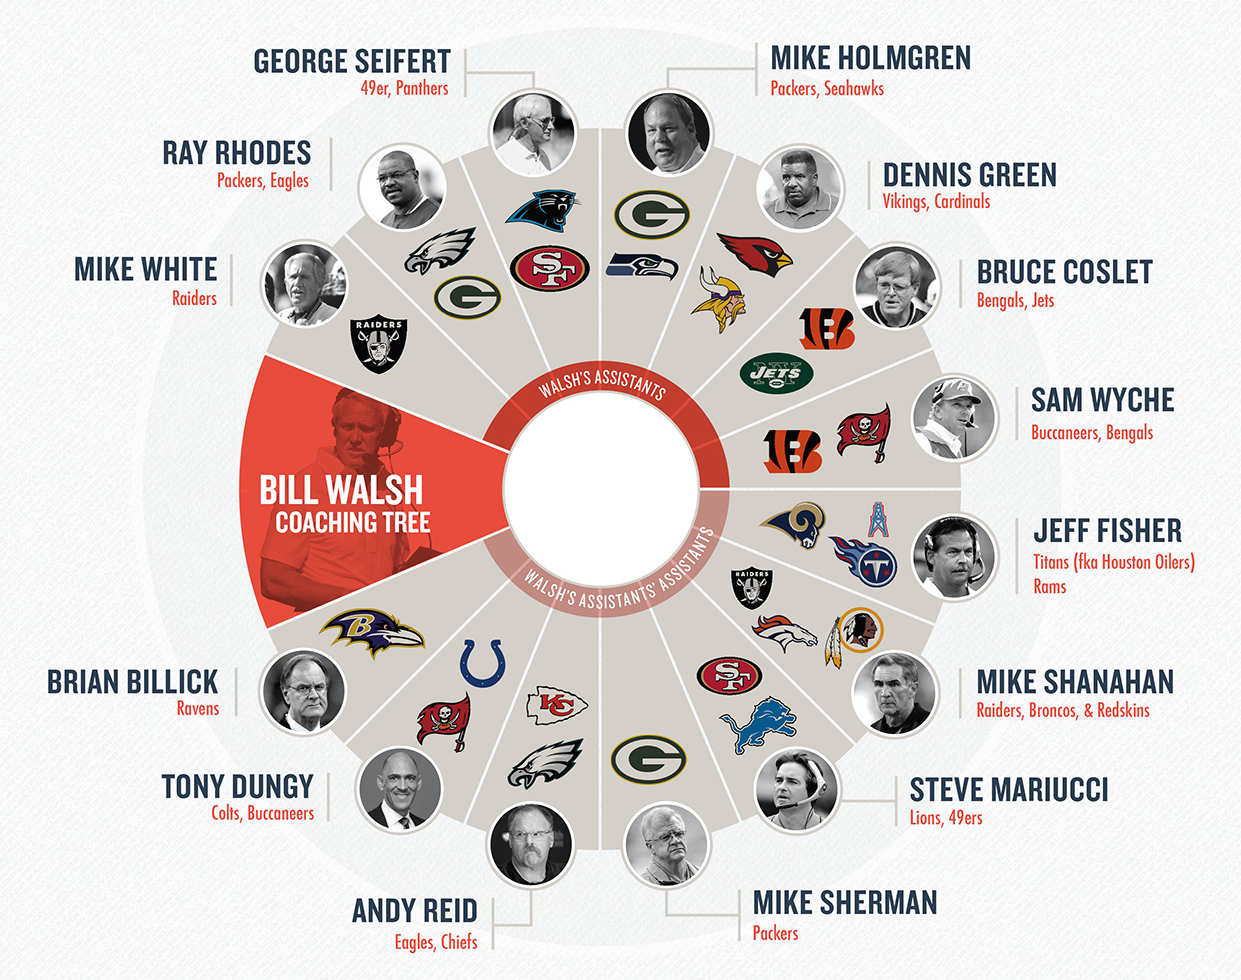
\includegraphics[width=\textwidth]{walsh_network.png}
\end{center}
\caption{Image: The Bill Walsh Coaching Tree. Source:
\url{http://blog.hubspot.com/marketing/paypal-mafia-bill-walsh-nfl-infographic}}
\label{fig-bill-walsh}
\end{figure}

This report considers a two main questions about NFL coaches who have worked
together.  First, does centrality in the social network align with overall
coaching success?  Second, are there distinct communities in the network,
perhaps aligned with some particular style or philosophy?

\section{Methodology}

\subsection{Data Acquisition}

Data on NFL coaching staffs was gathered from the site
\url{http://www.pro-football-reference.org} by reading the pages and parsing
the listed coaching staff.  For example, this page
\url{http://www.pro-football-reference.com/teams/det/2010.htm} lists the
coaches for the 2010 Detroit Lions.  The team page generally lists the head
coach, offensive coordinator, and defensive coordinator.  Only the years
1980-2013 were considered.  The code used to produce this data is available at \cite{scraper}.

\subsection{Network Construction}

The relationship between members of the coaching staff is subject to
interpretation.  Within this data, the coach may be both a coordinator and head
coach.  

For this analysis, I consider two constructions of the social network:
\begin{enumerate}

\item The first model attempts to follow the ``coaching family tree''
perception, and only has directed edges from head coach to coordinator.  This
approach attempts to model the influence of successful coaches through the
success of their assistants.  Edges are between the head coach and the
coordinators; coordinators have no connection to each other.  This model will
be referred to as the \emph{tree} model.  The tree model is used for centrality
measures since this report is looking for the centrality successful
\emph{head} coaches.  The file is {\tt coaches\_tree.gml}.

\item The second model considers each member of the staff to be connected with
every coach they served with, with increasing weight for each year served.
This approach attempts to identify coaching ``communities'' who may tend serve
together.  This model will be referred to as the \emph{peer} model.  The file
is {\tt coaches\_peer.gml}.

\end{enumerate}

\subsection{Analysis}

Network analysis is done in the R programming language with the {\tt igraph}
package.  The calculations are included in this document using the {\tt knitr}
package.

For centrality measurement, the validation metric is based on alignment with
super-bowl winning coaches since this data was easy to gather.  Due to multiple
career wins, there are only 23 super-bowl winning coaches since 1980.  Ideally
the evaluation should be based on a more continuous metric applicable to all
coaches, such as win percentage, which can be used to calculate correlation.

For community finding, it's difficult to pick a validation metric.  The main
evaluation metric is subjective based on the infographic in figure
\ref{fig-bill-walsh}.

\subsection{Limitations}

There are several important limitations of this analysis:

\begin{itemize}

\item Only the head coach and coordinators are considered.  This represents the
only clean data available from \url{http://pro-football-reference.com}.  It
also avoids the complexities resulting from teams having different names for
the various position coaches.  This has the downside of not recognizing cases
where head coaches and coordinators take jobs as position coaches.

\item Only the years 1980-2013 are considered.  The consistent reporting of
offensive and defensive coordinators appears to start around 1980.  This
results in the network being truncated for coaches employed before and after
1980.

\item Coaches are considered to serve the entire year.  In reality, teams may
occasionally fire coaches mid-year, and coaches may take a leave of absence.


\end{itemize}

\section{Network Properties}

The network includes 427 nodes.  The tree model has 777 edges; the peer model
has 1244.  In both networks, the possible number of edges is constrained due to
the realities of the coaching profession.  It's nearly impossible for a node to
have 0 edges since no coach serves all three roles.  The maximum degree is also
relatively limited due to coaching careers being finite.  It's rare for a head
coach or coordinator to be under 30 or over 70.



The degree distribution for the tree model is calculated as follows and shown in figure \ref{fig:tree-prop}.

\begin{knitrout}
\definecolor{shadecolor}{rgb}{0.969, 0.969, 0.969}\color{fgcolor}\begin{kframe}
\begin{alltt}
\hlstd{tree_g} \hlkwb{=} \hlkwd{read.graph}\hlstd{(}\hlstr{"coaches_tree.gml"}\hlstd{,}\hlkwc{format}\hlstd{=}\hlstr{"gml"}\hlstd{)}
\hlkwd{summary}\hlstd{(tree_g)}
\end{alltt}
\begin{verbatim}
## IGRAPH U--- 427 777 -- 
## attr: href (v/c), guid (v/c), label (v/c), id (v/n), value (e/n)
\end{verbatim}
\begin{alltt}
\hlstd{tree_deg} \hlkwb{=} \hlkwd{degree.distribution}\hlstd{(tree_g,} \hlkwc{cumulative} \hlstd{=} \hlnum{TRUE}\hlstd{)}
\hlkwd{plot}\hlstd{(tree_deg,}\hlkwc{log}\hlstd{=}\hlstr{"xy"}\hlstd{,}\hlkwc{xlab}\hlstd{=}\hlstr{"degree k"}\hlstd{,}\hlkwc{ylab}\hlstd{=}\hlstr{"P(x) >= k"}\hlstd{,}\hlkwc{cex}\hlstd{=}\hlnum{0.5}\hlstd{)}
\end{alltt}
\end{kframe}\begin{figure}

{\centering \includegraphics[width=\maxwidth]{figure/tree-prop-1} 

}

\caption[Cumulative degree distribution for tree model]{Cumulative degree distribution for tree model\label{fig:tree-prop}}
\end{figure}


\end{knitrout}

The degree distribution for the peer model is calculated as follows and shown
in figure \ref{fig:tree-prop}.

\begin{knitrout}
\definecolor{shadecolor}{rgb}{0.969, 0.969, 0.969}\color{fgcolor}\begin{kframe}
\begin{alltt}
\hlstd{peer_g} \hlkwb{=} \hlkwd{read.graph}\hlstd{(}\hlstr{"coaches_peer.gml"}\hlstd{,}\hlkwc{format}\hlstd{=}\hlstr{"gml"}\hlstd{)}
\hlkwd{summary}\hlstd{(peer_g)}
\end{alltt}
\begin{verbatim}
## IGRAPH U--- 427 1244 -- 
## attr: href (v/c), guid (v/c), label (v/c), id (v/n), value (e/n)
\end{verbatim}
\begin{alltt}
\hlstd{peer_deg} \hlkwb{=} \hlkwd{degree.distribution}\hlstd{(tree_g,} \hlkwc{cumulative} \hlstd{=} \hlnum{TRUE}\hlstd{)}
\hlkwd{plot}\hlstd{(peer_deg,}\hlkwc{log}\hlstd{=}\hlstr{"xy"}\hlstd{,}\hlkwc{xlab}\hlstd{=}\hlstr{"degree k"}\hlstd{,}\hlkwc{ylab}\hlstd{=}\hlstr{"P(x) >= k"}\hlstd{,}\hlkwc{cex}\hlstd{=}\hlnum{0.5}\hlstd{)}
\end{alltt}
\end{kframe}

{\centering \includegraphics[width=\maxwidth]{figure/peer-prop-1} 

}



\end{knitrout}

XXX

A Fruchterman-Reingold layout of the tree graph is show in figure
\ref{fig:graph-plot}.  There graph appears tightly clustered in general, without
an obvious community structure.

\begin{knitrout}
\definecolor{shadecolor}{rgb}{0.969, 0.969, 0.969}\color{fgcolor}\begin{kframe}
\begin{alltt}
\hlkwd{plot.igraph}\hlstd{(tree_g,} \hlkwc{layout}\hlstd{=layout.fruchterman.reingold,} \hlkwc{vertex.label}\hlstd{=}\hlnum{NA}\hlstd{,} \hlkwc{vertex.size}\hlstd{=}\hlnum{4}\hlstd{)}
\end{alltt}
\end{kframe}\begin{figure}

{\centering \includegraphics[width=\maxwidth]{figure/graph-plot-1} 

}

\caption[Visualization of the tree model]{Visualization of the tree model\label{fig:graph-plot}}
\end{figure}


\end{knitrout}

\section{Centrality}

There are several measures of centrality; it's unclear which is most useful for
this network.  This section considers \emph{betweenness}, \emph{closeness},
\emph{page rank}, and \emph{authority}.  The tree model is used in order to
stress the influence of the head coach.

\subsection{Degree}

The simplest centrality measure is degree centrality.  The following snippet
selects the top 20 nodes by degree:

\begin{knitrout}
\definecolor{shadecolor}{rgb}{0.969, 0.969, 0.969}\color{fgcolor}\begin{kframe}
\begin{alltt}
\hlstd{td} \hlkwb{=} \hlkwd{degree}\hlstd{(tree_g)}
\hlstd{top} \hlkwb{=} \hlkwd{V}\hlstd{(tree_g)}\hlopt{$}\hlstd{label[}\hlkwd{order}\hlstd{(td,} \hlkwc{decreasing}\hlstd{=}\hlnum{TRUE}\hlstd{)[}\hlnum{1}\hlopt{:}\hlnum{20}\hlstd{]]}
\hlkwd{intersect}\hlstd{(top, sb_winners)}
\end{alltt}
\begin{verbatim}
## [1] "Mike Shanahan"  "Mike Holmgren"  "Pete Carroll"   "Tom Coughlin"  
## [5] "George Seifert" "Bill Belichick" "Tony Dungy"
\end{verbatim}
\end{kframe}
\end{knitrout}

There are 7 Super Bowl winners in the top 20 nodes by degree centrality.

\subsection{Betweenness}

The first measure of centrality to be evaluated is betweenness, which measures
how many shortest paths traverse the node.  The following snippet calculates
betweenness for all nodes in the tree model and selects the 20 nodes with the
top betweenness.  

\begin{knitrout}
\definecolor{shadecolor}{rgb}{0.969, 0.969, 0.969}\color{fgcolor}\begin{kframe}
\begin{alltt}
\hlstd{bb} \hlkwb{=} \hlkwd{betweenness}\hlstd{(tree_g,} \hlkwc{v}\hlstd{=}\hlkwd{V}\hlstd{(tree_g),} \hlkwc{directed}\hlstd{=}\hlnum{TRUE}\hlstd{)}
\hlstd{top} \hlkwb{=} \hlkwd{V}\hlstd{(tree_g)}\hlopt{$}\hlstd{label[}\hlkwd{order}\hlstd{(bb,} \hlkwc{decreasing}\hlstd{=}\hlnum{TRUE}\hlstd{)[}\hlnum{1}\hlopt{:}\hlnum{20}\hlstd{]]}
\hlkwd{intersect}\hlstd{(top, sb_winners)}
\end{alltt}
\begin{verbatim}
## [1] "George Seifert" "Tom Coughlin"   "Bill Cowher"    "Mike Shanahan" 
## [5] "Pete Carroll"   "Mike Holmgren"
\end{verbatim}
\end{kframe}
\end{knitrout}

There are 6 super-bowl-winning coaches in the top 20.  Since there are 427
coaches in the graph and 23 Super Bowl winners, this is a promising result.

\subsection{Closeness}

Another measure of centrality is closeness, which represents the distance to
other nodes in the network.  The following snippet applies the closeness
calculation.

\begin{knitrout}
\definecolor{shadecolor}{rgb}{0.969, 0.969, 0.969}\color{fgcolor}\begin{kframe}
\begin{alltt}
\hlstd{cc} \hlkwb{=} \hlkwd{closeness}\hlstd{(tree_g,} \hlkwc{v}\hlstd{=}\hlkwd{V}\hlstd{(tree_g),} \hlkwc{mode}\hlstd{=}\hlstr{"out"}\hlstd{)}
\hlstd{top} \hlkwb{=} \hlkwd{V}\hlstd{(tree_g)}\hlopt{$}\hlstd{label[}\hlkwd{order}\hlstd{(cc,} \hlkwc{decreasing}\hlstd{=}\hlnum{TRUE}\hlstd{)[}\hlnum{1}\hlopt{:}\hlnum{20}\hlstd{]]}
\hlkwd{intersect}\hlstd{(top, sb_winners)}
\end{alltt}
\begin{verbatim}
## [1] "Bill Cowher"    "Mike Holmgren"  "George Seifert" "Mike Shanahan"
\end{verbatim}
\end{kframe}
\end{knitrout}

The result is 4 Super Bowl winners in the top 20, better than chance, but not
as strong as degree.

\subsection{Page Rank}

Page Rank is an algorithm developed at Google for ranking web pages based on
hyperlink structure \cite{pagerank}.  Each page's rank is based on the rank of
the pages that link to it.  This algorithm may help identify successful and
influential coaches in a way that other centrality measures don't.  Page Rank
is calculated in R as follows:

\begin{knitrout}
\definecolor{shadecolor}{rgb}{0.969, 0.969, 0.969}\color{fgcolor}\begin{kframe}
\begin{alltt}
\hlstd{pr}  \hlkwb{=} \hlkwd{page.rank}\hlstd{(tree_g)}\hlopt{$}\hlstd{vector}
\hlstd{top} \hlkwb{=} \hlkwd{V}\hlstd{(tree_g)}\hlopt{$}\hlstd{label[}\hlkwd{order}\hlstd{(pr,} \hlkwc{decreasing}\hlstd{=}\hlnum{TRUE}\hlstd{)[}\hlnum{1}\hlopt{:}\hlnum{20}\hlstd{]]}
\hlkwd{intersect}\hlstd{(top, sb_winners)}
\end{alltt}
\begin{verbatim}
## [1] "Tom Coughlin"   "Pete Carroll"   "Mike Shanahan"  "Bill Belichick"
## [5] "Mike Holmgren"  "George Seifert"
\end{verbatim}
\end{kframe}
\end{knitrout}

Again we find 6 Super Bowl winners in the top 20, indicating page rank is
reflective of coaching success.

\subsection{Kleinburg Authority/Hub}

Kleinberg's authority score is also based on web page hyperlinks
\cite{authority}.  Like Page Rank, it may be a more accurate centrality measure
that more crude measures.  It is calculated in R as follows:
\begin{knitrout}
\definecolor{shadecolor}{rgb}{0.969, 0.969, 0.969}\color{fgcolor}\begin{kframe}
\begin{alltt}
\hlstd{as} \hlkwb{=} \hlkwd{authority.score}\hlstd{(tree_g)}\hlopt{$}\hlstd{vector}
\hlstd{top} \hlkwb{=} \hlkwd{V}\hlstd{(tree_g)}\hlopt{$}\hlstd{label[}\hlkwd{order}\hlstd{(as,} \hlkwc{decreasing}\hlstd{=}\hlnum{TRUE}\hlstd{)[}\hlnum{1}\hlopt{:}\hlnum{20}\hlstd{]]}
\hlkwd{intersect}\hlstd{(top, sb_winners)}
\end{alltt}
\begin{verbatim}
## [1] "Mike Shanahan"  "Mike Holmgren"  "Bill Cowher"    "George Seifert"
## [5] "Mike McCarthy"
\end{verbatim}
\end{kframe}
\end{knitrout}

The top 20 nodes by Kleinberg authority score include only 5 Super Bowl winners.

\section{Community Structure}

In addition to centrality, the community structure of the NFL coaches network
may reflect intuitions around coaching 'families'.  

% cliques
\begin{knitrout}
\definecolor{shadecolor}{rgb}{0.969, 0.969, 0.969}\color{fgcolor}\begin{kframe}
\begin{alltt}
\hlstd{clq} \hlkwb{=} \hlkwd{largest.cliques}\hlstd{(}\hlkwd{as.undirected}\hlstd{(peer_g))}
\hlkwd{V}\hlstd{(peer_g)}\hlopt{$}\hlstd{label[clq[[}\hlnum{1}\hlstd{]]]}
\end{alltt}
\begin{verbatim}
## [1] "Mike Pettine"         "Rex Ryan"             "Brian Schottenheimer"
## [4] "Dennis Thurman"
\end{verbatim}
\end{kframe}
\end{knitrout}

First we consider k-cores:

% k-core
\begin{knitrout}
\definecolor{shadecolor}{rgb}{0.969, 0.969, 0.969}\color{fgcolor}\begin{kframe}
\begin{alltt}
\hlstd{cn} \hlkwb{=} \hlkwd{graph.coreness}\hlstd{(}\hlkwd{as.undirected}\hlstd{(peer_g))}
\hlstd{cn[}\hlkwd{which.max}\hlstd{(cn)]}
\end{alltt}
\begin{verbatim}
## [1] 5
\end{verbatim}
\begin{alltt}
\hlkwd{length}\hlstd{(cn[cn} \hlopt{==} \hlnum{5}\hlstd{])}
\end{alltt}
\begin{verbatim}
## [1] 116
\end{verbatim}
\end{kframe}
\end{knitrout}

The largest k-core is only 5 nodes, though 116 nodes belong to a 5-core.

\section{Conclusion}

This report analyzed the social network of NFL coaches serving as head coach or
coordinator in the years 1980-2013.  The two primary questions answered were
regarding the alignment of centrality measures with coaching success and the
existence of communities revolving around particular coaching styles and/or
philosophies.

With respect to centrality, this report finds that multiple centrality measures
were well-aligned with coaching success.  In the tree model, for both
betweenness and page rank, the top 20 vertices contained 6 super-bowl-winning
coaches.  This should not be surprising since winning coaches will tend to
coach for a long time and have their assistants hired away for other jobs,
leading to more edges.

With respect to communities, the results were less clear XXX.

The content used to generate this report can be found at \cite{project}.

\begin{thebibliography}{99}

\bibitem{mobility1} Harrison, C.K. \& Associates (2013). Coaching Mobility (Volume I in the Good Business Series). A Report for the NFL Diversity and Inclusion Series.

\bibitem{mobility3} Harrison, C.K. \& Bukstein, S. (2014). NFL Occupational Mobility Patterns (Volume III). A report for the NFL Diversity and Inclusion “Good Business” Series.

\bibitem{forbes-pay}  \url{http://www.forbes.com/sites/chrissmith/2013/05/22/the-highest-paid-coaches-in-us-sports/}

\bibitem{scraper} \url{https://github.com/ndire/pfr-scraper}

\bibitem{project} \url{https://github.com/ndire/sna-nfl-coaches}

\bibitem{pagerank} Sergey Brin and Larry Page: The Anatomy of a Large-Scale Hypertextual Web Search Engine. Proceedings of the 7th World-Wide Web Conference, Brisbane, Australia, April 1998.

\bibitem{authority} J. Kleinberg. Authoritative sources in a hyperlinked environment. Proc. 9th ACM-SIAM Symposium on Discrete Algorithms, 1998. Extended version in Journal of the ACM 46(1999). Also appears as IBM Research Report RJ 10076, May 1997.

\end{thebibliography}

\end{document}
